\documentclass[a3,portrait]{a0poster}
\nonstopmode
%\documentclass[portrait]{a0poster}
%\documentclass[a0poster]{article}

\usepackage[T1]{fontenc}
%\usepackage[koi8-r]{inputenc}
\usepackage[latin1]{inputenc}
%\usepackage[utf8]{inputenc}
%\usepackage[russian]{babel}
%\usepackage[french]{babel}
\usepackage[english]{babel}
%\usepackage[T1]{fontenc}



\usepackage{pbsi}
%\usepackage{mathptmx}
%\usepackage{tgothic}
%\usepackage{vicent}
\usepackage{chancery}
\usepackage{fourier}


\usepackage{eso-pic}
\usepackage[pdftex]{graphicx}
\usepackage[usenames,dvipsnames]{color}
%\usepackage{color}
%\usepackage[dvipsnames]{color}



\definecolor{MyDarkBlue}{rgb}{0,0.08,0.45}
\definecolor{IITPLightBlue}{rgb}{0.27,0.45,0.73}
\definecolor{IITPBlue}{rgb}{0.25,0.41,0.68}
\definecolor{IITPDarkBlue}{rgb}{0.19,0.32,0.50}
\definecolor{IITPDarkDarkBlue}{rgb}{0.15,0.24,0.37}
%\definecolor{MyDarkGreen}{rgb}{0,0.3,0}
\definecolor{MyDarkGreen}{rgb}{0.3,0.5,0.2}
\input dvipsnam.def
%\usepackage[OT1]{fontenc}
\usepackage[T1]{fontenc}


%\usepackage{nimbus}
%\renewcommand*\familydefault{\sfdefault} %% Only if the base font of the document is to be sans serif
%\usepackage[T1]{fontenc}

\newcommand\notyet[1]{ }

\oddsidemargin -1.5cm
\textwidth 28cm
\textheight 38cm

%\oddsidemargin 15mm
%\evensidemargin 15mm
%\topmargin -5mm

\setlength{\parindent}{-5mm}
\setlength{\parskip}{2pt}

%\setlength{\baselineskip}{10pt}

\pagestyle{empty}

\providecommand{\LenToUnit}[1]{#1\@gobble}
\newcommand{\PRH}[5]{%
\AddToShipoutPicture*{\put(\LenToUnit{#3},\LenToUnit{#4}){%
     \parbox[b][\paperheight]{\paperwidth}{%       
       \vfill
       \centering
       \includegraphics[width=#1,height=#2,%
                        keepaspectratio]{#5}%
       \vfill
     }}}
}  

\newcommand\BackgroundStrip{
\put(-8,420){
\parbox[b][\paperheight]{\paperwidth}{%
\vfill
\centering
\vfill
}}}

\newcommand\BackgroundPic{
%\put(-4,0){
\put(-8,-60){
\parbox[b][\paperheight]{\paperwidth}{%
\vfill
\centering
%%AC: takes a lot of time:
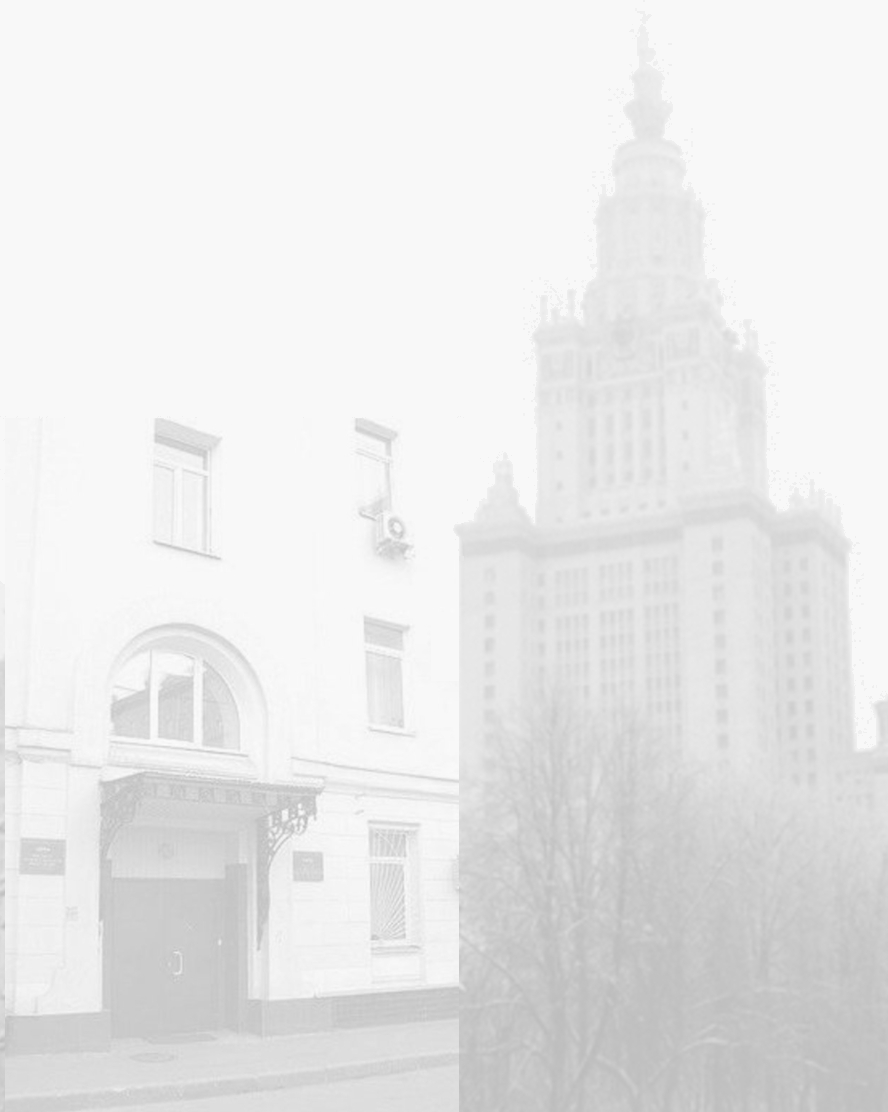
\includegraphics{background-poster.png}%
\vfill
}}}


\begin{document}

\footnotesize

\AddToShipoutPicture{\BackgroundStrip}

\AddToShipoutPicture{\BackgroundPic}

\notyet
{\bsifamily
\footnotesize
\color{GreenYellow}GreenYellow
\color{Yellow}Yellow
\color{Goldenrod}Goldenrod
\color{Dandelion}Dandelion
\color{Apricot}Apricot
\color{Peach}Peach
\color{Melon}Melon
\color{YellowOrange}YellowOrange
\color{Orange}Orange

\color{BurntOrange}BurntOrange
\color{Bittersweet}Bittersweet
\color{RedOrange}RedOrange
\color{Mahogany}Mahogany
\color{Maroon}Maroon
\color{BrickRed}BrickRed
\color{Red}Red
\color{OrangeRed}OrangeRed

\color{RubineRed}RubineRed
\color{WildStrawberry}WildStrawberry
\color{Salmon}Salmon
\color{CarnationPink}CarnationPink
\color{Magenta}Magenta
\color{VioletRed}VioletRed
\color{Rhodamine}Rhodamine

\color{Mulberry}Mulberry
\color{RedViolet}RedViolet
\color{Fuchsia}Fuchsia
\color{Lavender}Lavender
\color{Thistle}Thistle
\color{Orchid}Orchid
\color{DarkOrchid}DarkOrchid
\color{Purple}Purple
\color{Plum}Plum

\color{Violet}Violet
\color{RoyalPurple}RoyalPurple
\color{BlueViolet}BlueViolet
\color{Periwinkle}Periwinkle
\color{CadetBlue}CadetBlue
\color{CornflowerBlue}CornflowerBlue
\color{MidnightBlue}MidnightBlue

\color{NavyBlue}NavyBlue
\color{RoyalBlue}RoyalBlue
\color{Blue}Blue
\color{Cerulean}Cerulean
\color{Cyan}Cyan
\color{ProcessBlue}ProcessBlue
\color{SkyBlue}SkyBlue
\color{Turquoise}Turquoise
\color{TealBlue}TealBlue

\color{Aquamarine}Aquamarine
\color{BlueGreen}BlueGreen
\color{Emerald}Emerald
\color{JungleGreen}JungleGreen
\color{SeaGreen}SeaGreen
\color{Green}Green
\color{ForestGreen}ForestGreen
\color{PineGreen}PineGreen

\color{LimeGreen}LimeGreen
\color{YellowGreen}YellowGreen
\color{SpringGreen}SpringGreen
\color{OliveGreen}OliveGreen
\color{RawSienna}RawSienna
\color{Sepia}Sepia
\color{Brown}Brown
\color{Tan}Tan
\color{Gray}Gray

\vskip -7.25cm
%\end{document}

}%\notyet



\begin{center}

%\vskip -50mm

\ \vskip -1.2cm


%\color{MyDarkGreen}
%\color{Sepia}
%\color{ForestGreen}
%\color{Mahogany}
\color{IITPBlue}
%\color{IITPBlue}
%\begin{array}{c}
%\mbox{
%\bfseries\huge
%\titlefontlarge
%\tgothfamily\huge
{\bfseries\LARGE
Differential Equations and Applications
}

\vskip 0.6cm

%\color{Mahogany}
\color{IITPLightBlue}
%\color{Sepia}
{%\titlefont
%\bsifamily\small
%\itshape
%\hfill
\scshape\bf\large
%\qquad
International Conference
%}
%
%\vskip 0.3cm
%
%{
%\scshape\large\bf
in Honour of Mark Vishik
%\quad
}

\vskip 0.6cm

{
\bf\large
%\qquad\qquad\qquad\qquad
%\hfill
On the Occasion of his 90th Birthday
%\quad
}

\vskip 0.6cm

{\bf\large
%\qquad\qquad\qquad\qquad\qquad\qquad
%\hfill
Moscow, June 4-7, 2012
%\quad
}

\end{center}



\medskip

%\scriptsize
%\footnotesize
%\titlefontsmall
%\color{MyDarkBlue}
\color{IITPDarkBlue}
%\begin{tabular}{l}
%IITP RAS, Moscow, June 4-7, 2012
%\\


\PRH{300pt}{570pt}{-85mm}{15mm}{mi-749}

%\vskip 1cm

%\hskip 13.5cm
%{\speakerfont
%Fountain Hall, RAS, Vorobjevy gory (Monday, June 4)
%}

%\hskip 13.5cm
%{\speakerfont
%IITP, Bolshoj Karetny,\,19 (Tuesday\,--Thursday, June 5-7)
%}

%\vskip 2cm

%\hskip 14cm
%\hskip 3cm
%{\scshape
%The Borodin Quartet}

%{\itshape\scriptsize
%\hskip 14cm
%\hskip 0.5cm
%\begin{tabular}{l}
% Joseph Haydn, String Quartet Opus 33 No.\,2, E-flat major
%\\
%%Johannes Brahms, String Quartet Opus 51 No.\,1, C minor
%\end{tabular}
%}

%\vskip 2cm

%\hskip 14cm
%\hskip 4cm
%{\bsifamily Plenary speakers}

%\vskip -0.5cm

%\hskip 14cm
%\hskip 0.2cm
%{%\scriptsize
%\footnotesize
%\begin{tabular}{l}
%\\Mark Freidlin
%\\Alain Haraux
%\\Yulij Ilyashenko
%\\Sergei Kuksin
%\\Victor Maslov
%\\Stanislav Molchanov
%\\Nikolai Nadirashvili
%\end{tabular}
%\quad
%\begin{tabular}{l}
%\\Louis Nirenberg
%\\Stanislav Pohozhaev
%\\George Sell
%\\Alexander Shnirelman
%\\Roger Temam
%\\Edriss Titi
%\\Boris Vainberg
%\\Vladimir Zakharov
%\end{tabular}
%}

\vskip 0.9cm

\hskip 12cm
\hskip 5cm
{\bsifamily Invited speakers}

%\vskip 0.3cm

{
%\bfseries\tiny
\bf
%\tiny
%\footnotesize
\scriptsize
\hskip 12cm
%\hskip 15cm
\begin{tabular}{l}
\\Mikhail Agranovich
\\Anatoli Babin
\\Claude Bardos
\\Sergey Bezrodnykh
\\Vladimir Chepyzhov
\\Igor Chueshov
\\Alexander Demidov
\\Sergey Dobrokhotov
\\Stamatis Dostoglou
\\Julii Dubinskii
\\Alexander Dynin
\\Grigory Eskin
\\Mark Freidlin
\\Leonid Friedlander
\\Andrei Fursikov
\\Evgeny Gorin
\\Andrey Goritsky
\\Alexander Grigoryan
\\Nikolay Gusev
\\Alain Haraux
\\Valentina Ipatova
\\Yulij Ilyashenko
\\Alexei Ilyin
\\Valeriy Imaykin
\\Shoshana Kamin
\end{tabular}
\begin{tabular}{l}
\\Aleksey Kapustyan
\\Alexander Komech
\\Andrey Komech
\\Elena Kopylova
\\Alexander Krasnoselskii
\\Victor Kozyakin
\\Sergei Kuksin
\\Jean-Pierre Loh�ac
\\Andrey Lyapin
\\Mark Malamud
\\Victor Maslov
\\Alain Miranville
\\Stanislav Molchanov
%\end{tabular}
%\begin{tabular}{l}
\\Olga Mukina
\\Nikolai Nadirashvili
\\Louis Nirenberg
\\Alexander Ovseevich
\\Victor Palamodov
\\Boris Paneah
\\Vittorino Pata
\\Andrey Piatnitski
\\Stanislav Pohozhaev
\\Olga Pyrkova
\\Evgeny Radkevich
\\Nikita Ratanov
\end{tabular}
\begin{tabular}{l}
\\Igor Rudakov
\\George Sell
\\Bert-Wolfgang Schulze
\\Gregory Seregin
\\Andrei Shafarevich
\\Armen Shirikyan
\\Alexander Shnirelman
\\Mikhail Shubin
\\Yakov Sinai
\\Elena Sitnikova
\\Alexander Skubachevskii
\\Vsevolod Solonnikov
\\Tatiana Suslina
\\Nikolai Tarkhanov
\\Roger Temam
\\Edriss Titi
\\G�rard Tronel
\\Boris Vainberg
\\Vladimir Vlasov
\\Nikita Vvedenskaya
\\Wolfgang Wendland
\\Ingo Witt
\\Hisao Fujita Yashima
\\Vladimir Zakharov
\\Sergey Zelik
\end{tabular}
%\end{tabular}
}

\vskip 0.8cm

\hskip 13.5cm
{\bf\scriptsize
\begin{tabular}{l}
Chair of the Organizing Committee: Alexander Kuleshov
\\
Chair of the Scientific Committee: Andrei Fursikov
\\
With the support of IITP RAS, RFBR, and Moscow State University
\\
www.dynamics.iitp.ru/vishik
\end{tabular}
}


\vskip 0.8cm

\color{IITPBlue}

\hskip 4cm
\begin{tabular}{l}
{\bf\scshape
Monday, June 4:
plenary talks, concert, and dinner}
\\
{\bf\scshape
\quad
Special guests: The Borodin Quartet}
\\
{\bf\scshape
\quad
Fountain Hall, 
Russian Academy of Sciences, 
Leninskii Prospekt,\,32a
%Vorobyovy Gory
}
\\
\qquad\qquad
%{\bf\scshape\footnotesize
%Plenary talks, concert and dinner
%The Borodin Quartet}
%\\
%\qquad\qquad
%{\bf\scshape Banquet}
\\
{\bf\scshape
Tuesday, Wednesday, Thursday; June 5-7}
\\
\quad
{\bf\scshape
IITP, Bolshoi Karetny,\,19}
\end{tabular}

\vfill

\vskip -1cm

%\quad
\,
\includegraphics[height=30mm]{ippi-logo-en.png}
\hskip 7cm

\includegraphics[height=20mm]{rfbr-logo-en.png}
\hfill

\includegraphics[height=40mm]{msulogo-thin.png}
\qquad



\end{document}
